\documentclass{article}

\usepackage{listings}
\usepackage{graphicx}
\usepackage{color}
\usepackage{float}
\lstset{numbersep=5pt,numbers=left,numberstyle=\footnotesize,title=\lstname,basicstyle=\footnotesize,showspaces=false,breaklines=true}

\begin{document}

\title{Knapsack problem - Dynamic programming}

\author{Jander Nascimento}

\maketitle

\tableofcontents

\section{Recursive algorithm}

Here is the recursive algorithm\cite{algojava} that can be used to obtain the optimal value of the knapsack.

\begin{lstlisting}
//Max function that returns the biggest value among the two parameters passed.
recDP(int[] w,int[] p, int i, int j){
  if i=0 OR j=0 then 
    return 0;
  fi

  if w[i-1]>j then
    return recDP(w,p,i-1,j)
  fi

  if w[i-1]<=j then
    return Max(recDP(w,p,i-1,j),
 		p[i-1]+recDP(w,p,i-1,j-w[i-1])
  fi
}
\end{lstlisting}

The running cost of the algorithm is proportional to the number of itens. Mathematically, let's consider
the function T(n) the function that express the running time. Using T(n), we may define as 
T(n)=nW the running time and 0(nW) the space usage.

The formulation of the problem is the following:

\[
  A(i,j) = \left\{ 
  \begin{array}{l l}
    0 & \quad \textnormal{if $i$ = 0 or $j$ = 0}\\
    A(i-1,j) & \quad \textnormal{if $w_i$ \textgreater j}\\
    max\{A(i-1,j),v_i+A(i-1,j-w_i)\} & \quad \textnormal{if $w_i$ \textless= j}\\
  \end{array} \right.
\]

\section{Sequencial algorithm}          

In the sequencial algorithm(SeqDP) calculated the entire matrix of prices to choose which one is the best, this 
better than any other alternative avoids re-computing the values of the knapsack.

\begin{lstlisting}
//Max function that returns the biggest value among the two parameters passed.
//w array with weights
//p array with prices
//W knapsack maximum weight
//n total number of itens
seqDP(int w[],int p[],int W,int n){

  for i:=0 to W do
    knap[0][i]:=0
  od

  for k:=1 to n do
    knap[k][0]:=0
    for y:=1 to W do
      if y < w[k-1] then
        knap[k][y]:=knap[k-1][y]
      else
        knap[k][y]:=Max(knap[k-1][y],
			p[k-1]+knap[k-1][y-w[k-1]])
      fi

  return knap[n][W]

}
\end{lstlisting}


\section{Is Recovering the reason for optimal solution?}          

\section{SeqDP and RecDP \textit{versus} Brute-force and Greedy}

\subsection{Time analysis}

\begin{figure} [H]
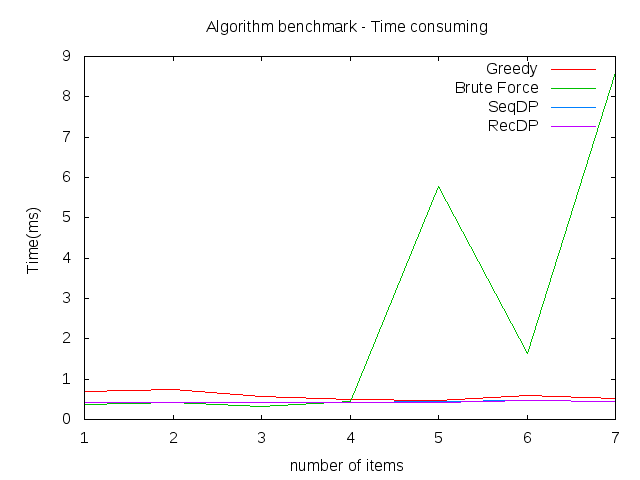
\includegraphics[scale=0.4]{report/time_analysis}
\caption{Algorithms comparison: timing}
\label{report/time_analysis}
\end{figure}

The chart above shows the run time behaviour of the algorithms Brute-Force, Greedy, SeqDP and RecDP. 
Accoding to the chart we can see that the algorithms Greedy, secDP and recDP, are much faster than brute-force algorithm.
We can see in a clear way the diffence between the three best algorithms by removing the Brute-Force, as shown: 

\begin{figure} [H]
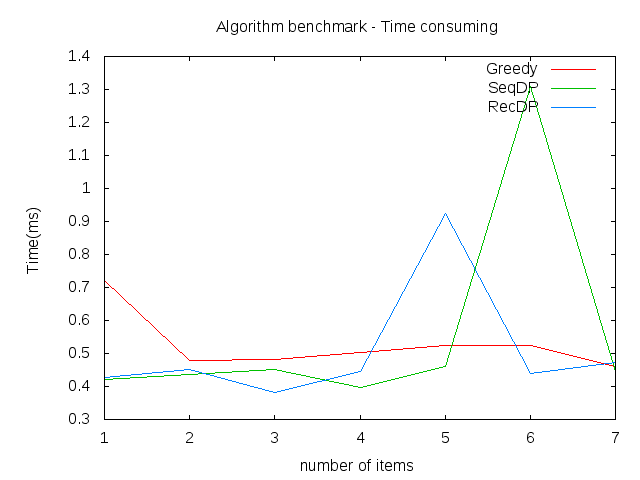
\includegraphics[scale=0.4]{report/time_analysis_no_bf}
\caption{Algorithms comparison,timing: Greedy, RecDP and SeqDP}
\label{report/time_analysis_no_bf}
\end{figure}

The Greedy algorithm might seems a good solution from this point of view, but as we are going to see in the next section, 
in term of efficiency the Greedy is not a good algorithm, since the value of the knapsack is not the optimal.

\subsection{Price analysis}

As the time is not the only contraint to be evaluated in the algorithm, the price of the knapsack can also be a variable
to be analyzed. Since this variable denotates how efficience the algorithm was, in terms of price.

\begin{figure} [H]
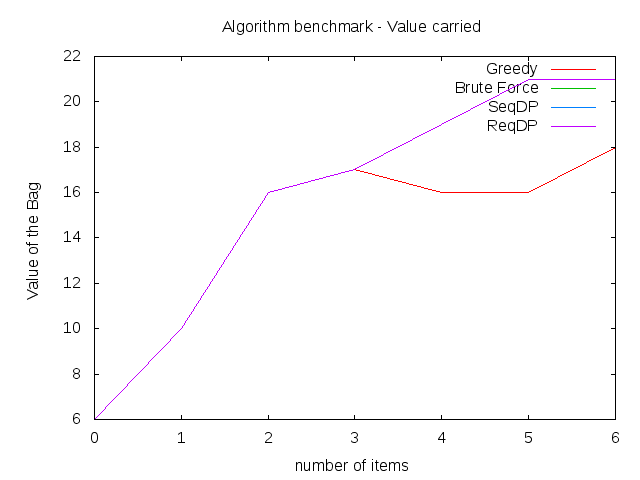
\includegraphics[scale=0.4]{report/price_analysis}
\caption{Algorithms comparison: price}
\label{report/price_analysis}
\end{figure}

As we can see in the chart above, the greedy algorithm with more than 3 itens provides a solution in which the value of the 
knapsack is not optimal if compared to Brute-Force, RecDP and SeqDP.

\subsection{What can i do within 30 sec}

As suggested in the subject, here was selected the best implementation, which is the seqDP, to perform the tests. By runnning SeqDP it is 
possible to find best solution for 50000 elements within 30 seconds.

\section{RecDP and array usage}

The test was performed with an instance of 10 itens and knapsack maximum weight of 64 shows that the total array size created was
640 and only 220 position were indeed used, this represents only 35\% of the array. This means that recursive approach evaluates
less subproblems than the sequencial approach.

\section{Better cases for RecDP}

Based on the fact that the recursive algorithm do not compute the entire table, we can predict the family in which the recursive is better
than the sequencial algorithm. 

The family of instances are those instances where we have bigger weights for the knapsack, this happens
because the sequencial algorithm must to compute the entire matrix (itens \textit{versus} weight) to find the result, while the recursive one
do not.

\begin{thebibliography}{9}

\bibitem{algojava}
  Robert Sedgewick,
  \emph{Algorithms in Java}.
  Addison-Wesley, 2002,
  3rd Edition,
  1994.

\end{thebibliography}

\end{document}
